% !TEX TS-program = pdflatex
% !TEX encoding = UTF-8 Unicode

% This is a simple template for a LaTeX document using the "article" class.
% See "book", "report", "letter" for other types of document.

\documentclass[11pt]{article} % use larger type; default would be 10pt

\usepackage[utf8]{inputenc} % set input encoding (not needed with XeLaTeX)
\usepackage{graphicx}
\graphicspath{ {image/} }
%%% Examples of Article customizations
% These packages are optional, depending whether you want the features they provide.
% See the LaTeX Companion or other references for full information.

%%% PAGE DIMENSIONS
\usepackage{geometry} % to change the page dimensions
\geometry{a4paper} % or letterpaper (US) or a5paper or....
% \geometry{margin=2in} % for example, change the margins to 2 inches all round
% \geometry{landscape} % set up the page for landscape
%   read geometry.pdf for detailed page layout information

\usepackage{graphicx} % support the \includegraphics command and options

% \usepackage[parfill]{parskip} % Activate to begin paragraphs with an empty line rather than an indent

%%% PACKAGES
\usepackage{booktabs} % for much better looking tables
\usepackage{array} % for better arrays (eg matrices) in maths
\usepackage{paralist} % very flexible & customisable lists (eg. enumerate/itemize, etc.)
\usepackage{verbatim} % adds environment for commenting out blocks of text & for better verbatim
\usepackage{subfig} % make it possible to include more than one captioned figure/table in a single float
% These packages are all incorporated in the memoir class to one degree or another...

%%% HEADERS & FOOTERS
\usepackage{fancyhdr} % This should be set AFTER setting up the page geometry
\pagestyle{fancy} % options: empty , plain , fancy
\renewcommand{\headrulewidth}{0pt} % customise the layout...
\lhead{}\chead{}\rhead{}
\lfoot{}\cfoot{\thepage}\rfoot{}
\usepackage{listings}

%%% SECTION TITLE APPEARANCE
\usepackage{sectsty}
\allsectionsfont{\sffamily\mdseries\upshape} % (See the fntguide.pdf for font help)
% (This matches ConTeXt defaults)

%%% ToC (table of contents) APPEARANCE
\usepackage[nottoc,notlof,notlot]{tocbibind} % Put the bibliography in the ToC
\usepackage[titles,subfigure]{tocloft} % Alter the style of the Table of Contents
\renewcommand{\cftsecfont}{\rmfamily\mdseries\upshape}
\renewcommand{\cftsecpagefont}{\rmfamily\mdseries\upshape} % No bold!

%%% END Article customizations

%%% The "real" document content comes below...

\title{CS770: Assignment 3}
\author{Ronghao Yang\\ID:20511820}
%\date{} % Activate to display a given date or no date (if empty),
         % otherwise the current date is printed 

\begin{document}
\maketitle

\section{Question 1}
\subsection{Question 1a}
\begin{lstlisting}[language=Octave]
function [X,errors] = newtons(f,d,x0,tol,maxiter)
% f is the input function, in our implementation, it's a string
% d is the input derrivative, in our implementation, it's a string
% x0 is the initial guess of the root
% tol is the error tollerance
% maxiter is the maximum iteration

    switch nargin
        case 3
            tol = 10^-4;
            maxiter = 10000;
        case 4
            tol = 10^-4;
    end
    % the default tollerence is set to be 10^-4
    % the default maximum iteration is set to be 10000
    
    f = inline(f);
    d = inline(d);
    %change the text version of the function and derrivative
    %to numerical version
    
    X = [];
    X = [X x0];
    errors = [];
    x1 = x0 - f(x0)./d(x0);
    X = [X x1];
    errors = [errors abs(x1-x0)];
    
    k = 1;
    while  (errors(k) > tol) && (k <= maxiter)
        x0 = X(k+1);
        tempX = x0- f(x0)./d(x0);
        %calculate the next value
        errors = [errors abs(tempX - X(end))];
        X = [X tempX];
        k = k+1;
    end
        
end
\end{lstlisting}

\subsection{Question 1b}
In my Newton's method, I set the tolerance of error to be $10^{-4}$ and the maximum number of iteration to be $10^{4}$.
\subparagraph{•}
Newton's Method Converges Well: \\
\centerline{$f(x) = x^{2}-10x$, $d(x) = 2x-10$, $x_{0} = 11$}\\
\begin{center}
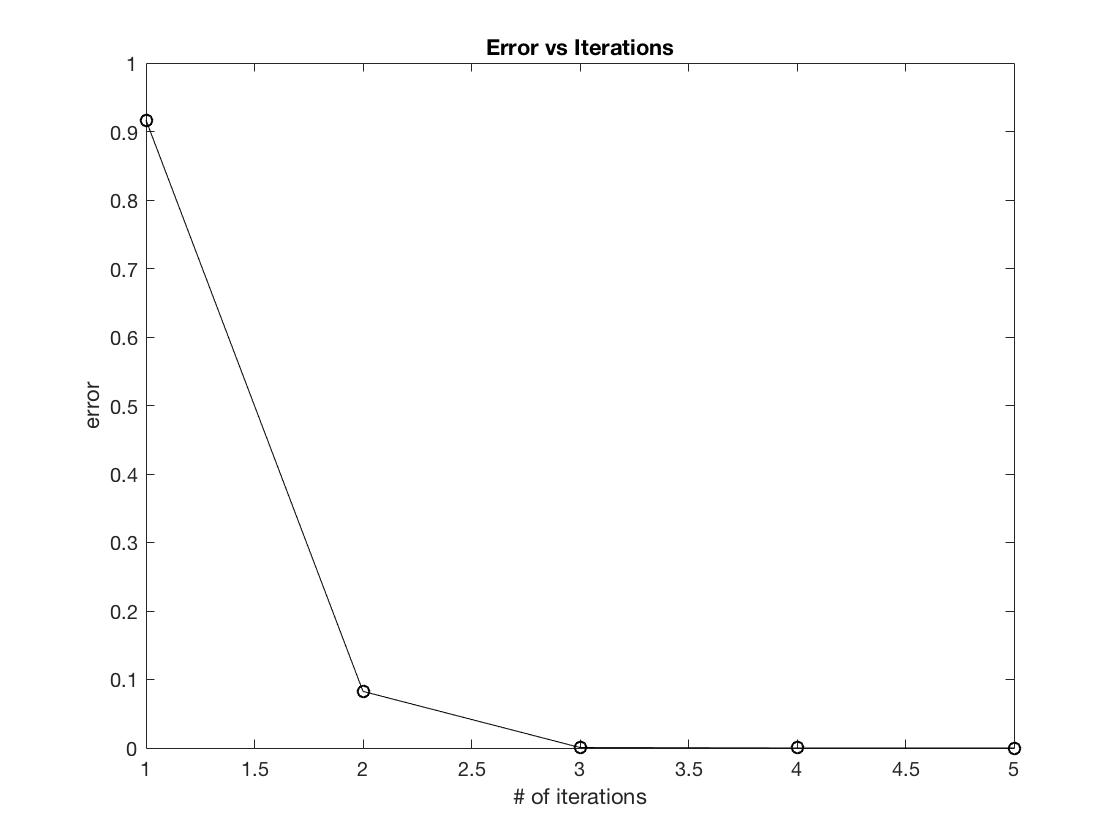
\includegraphics[scale = 0.35]{q121.jpg}
\end{center}
\subparagraph{•}
Newton's Method Doesn't Converges:\\\linebreak
\centerline{$f(x) = x^{2}+10$, $d(x) = 2x$}\\\\
Since $f(x)$ has no roots on its domain, whatever $x_{0}$ is chosen, $x$ won't converge.
\subparagraph{•}
Newton's Method Converges Slowly: \\\linebreak
\centerline{$f(x) = x^{20} - 100$, $d(x) = 20x^{19}$, $x_{0} = 100000000$}\\\\
\begin{center}
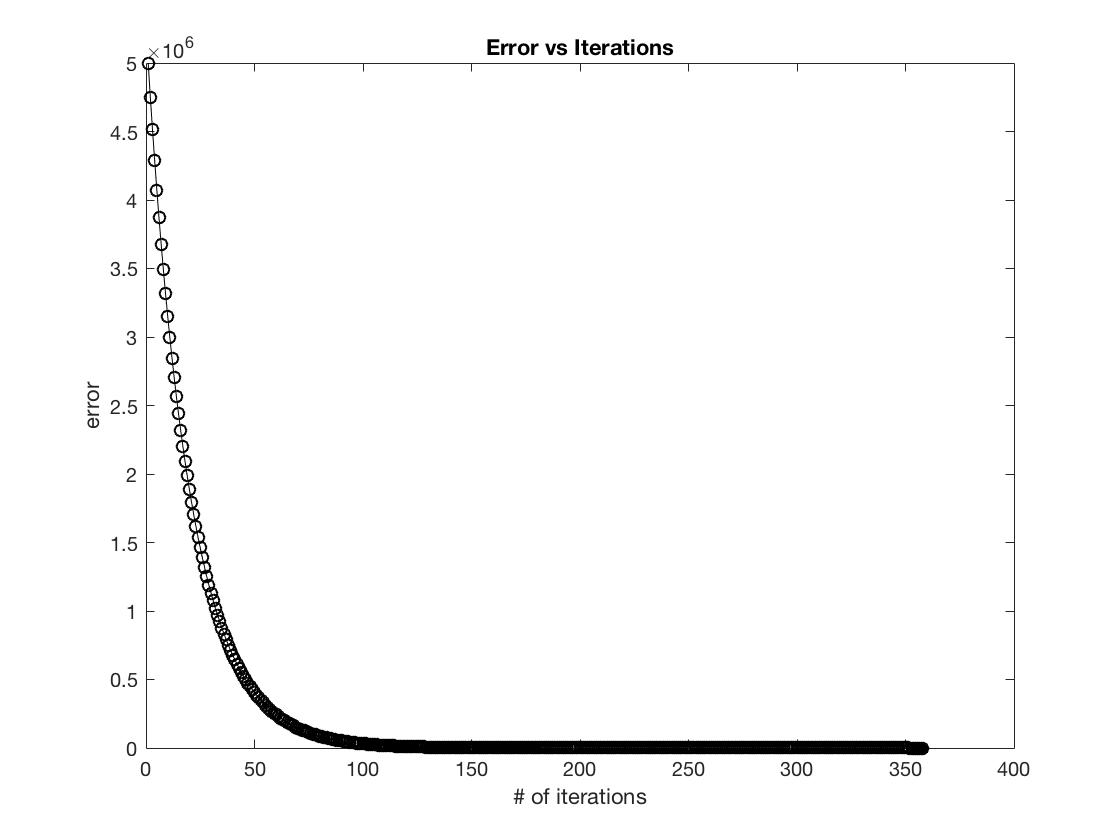
\includegraphics[scale = 0.35]{q123.jpg}
\end{center}
\section{Question 2}
\subsection{Question 2a}
\centerline{$f(x) = (x-1)^{2}e^{x}$, $d(x) = 2(x-1)e^{x}+(x-1)^{2}e^{x}$}
Therefore, when $x\neq1$, $d(x)\neq0$, therefore, Newton's iteration is well defined for $x\neq1$. \medskip

\centerline{$f(x^{*}) = f(x_{k})+(x^{*}-x_{k})f'(x_{k})+\frac{f''(\epsilon)(x^{*}-x_{k})^{2}}{2} = 0$}
\centerline{$x_{k+1}$ =  $x_{k}$ - $\frac{f(x_{k})}{d(x_{k})}$}
\centerline{$x_{k+1}$ - $x_{k}$ = - $\frac{f(x_{k})}{d(x_{k})}$}
\centerline{$f(x_{k})$ =$-(x_{k+1}$ - $x_{k})f'(x_{k})$, where $f'(x_{k}) = d(x_{k})$}
\centerline{$f(x^{*}) = f(x_{k})+(x^{*}-x_{k})f'(x_{k})+\frac{f''(\epsilon)(x^{*}-x_{k})^{2}}{2} = 0$ can be rewritten as}
\centerline{$f(x^{*}) = -(x_{k+1}$ - $x_{k})f'(x_{k}) + (x^{*}-x_{k})f'(x_{k})+\frac{f''(\epsilon)(x^{*}-x_{k})^{2}}{2} = 0$}
\centerline{$f(x^{*}) = (x^{*}-x_{k+1})f'(x_{k})+\frac{f''(\epsilon)(x^{*}-x_{k})^{2}}{2} = 0$}
\centerline{$\lim_{k\gets\infty}\frac{\mid e_{k+1}\mid}{\mid e_{k}\mid^{2}}$ = $\frac{f''(x^{*})}{2f'(x^{*})}$ = $C$}
Therefore, this is a second order method.\medskip
Beside, since $x_{k+1}$ = $\frac{x_{k}^{2}+1}{x_{k}+1}$, this method will converge slowly when x is big.
\subsection{Question 2b}
When $x_{0} = 2$,
\begin{center}
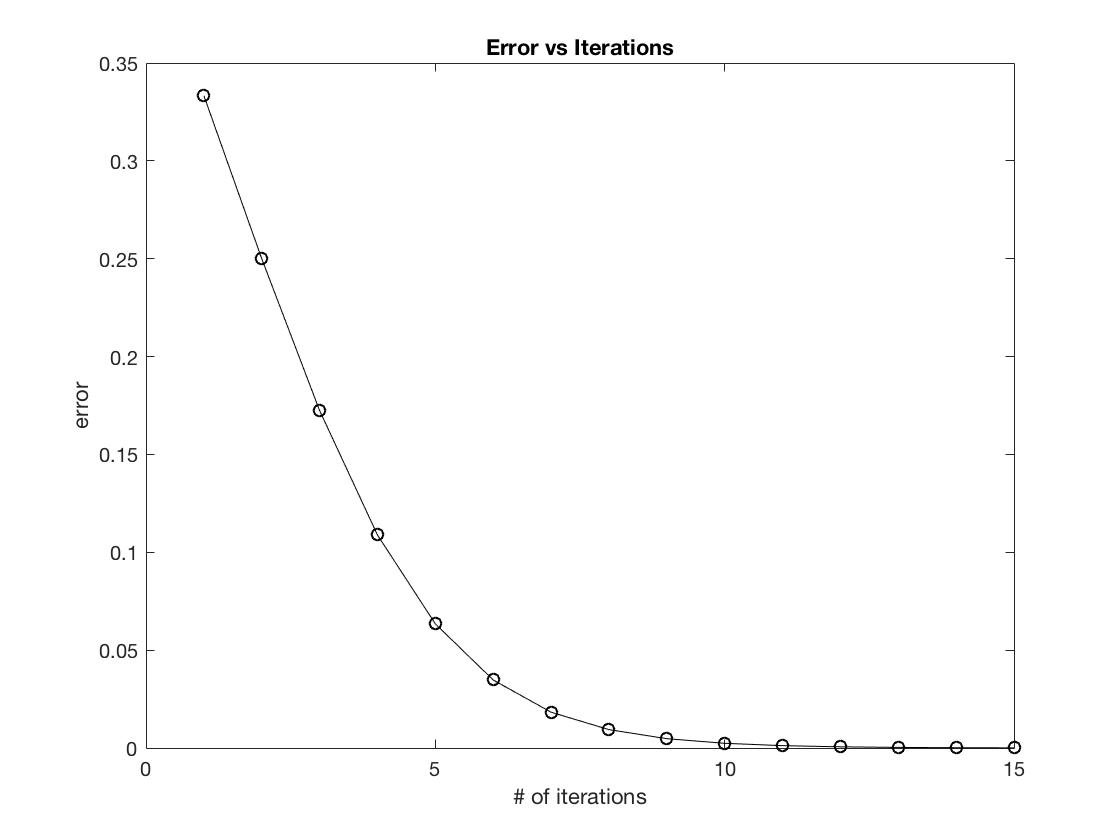
\includegraphics[scale = 0.35]{q22.jpg}\\\medskip
\end{center}
$\frac{f(x_{old})}{d(x_{old)}}$ can be written as $1-\frac{2}{x+1}$, let $s(x) = x - (1-\frac{2}{x+1})$, then $s(x) = \frac{x^{2}+1}{x+1}$, then $\frac{\partial}{\partial x}s(x)$=$1-\frac{2}{(x+1)^{2}}$, as we can see here, when x is large, $f(x)$ converges slowly, as $x$ decreases, $f(x)$ converges faster. 
\section{Question 3}
\subsection{Question 3a}
If a polynomial has a multiple root at $x^{*}$, then its derivative also has root(s) at $x^{*}$. If the multiplicity of root $x^{*}$ for polynomial $f(x)$ is $m$, then the multiplicity of root $x^{*}$ for $f'(x)$ is $m-1$. Therefore, the multiplicity of root $x^{*}$ for $w(x)$ = $f(x)$/$f'(x)$ is 1, so $w(x)$ has a simple root at $x^{*}$.
\subsection{Question 3b}
\centerline{$w(x)$ = $f(x)$/$f'(x)$, $w'(x)$ =$ \frac{f'(x)f'(x)-f(x)f''(x)}{f'(x)^2}$}\medskip
\centerline{For the update: $x$ = $x_{0} - w(x_{0})/w'(x_{0})$, where $x_{0}$ is the value before update}\medskip
\centerline{To simplify this equation, $x$ = $\frac{f(x)f'(x)}{f'(x)f'(x)-f(x)f''(x)}$}
\subsection{Question 3c}
\begin{center}
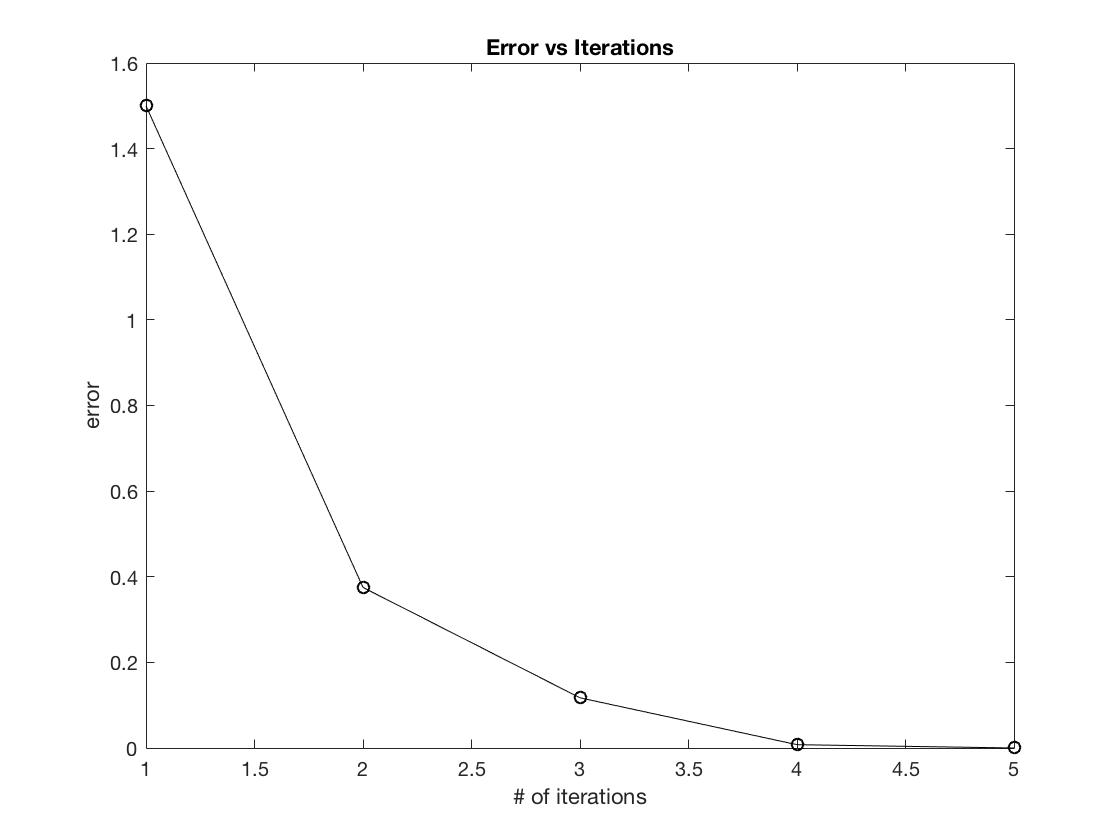
\includegraphics[scale = 0.35]{q33.jpg}\\\medskip
\end{center}
Compared to Newton's method, this method converges much faster, however, this method requires the computation of the second derivative which means more calculation is required.
\section{Question 4}
\paragraph{Proof:}\mbox{}\\
\centerline{$x^{k+1}$ =$x^{k}$ - $f(x^{k})$ $\frac{f(x^{k})}{f(x^{k}+f(x^{k}))-f(x^{k})}$}\\\linebreak
\centerline{Let $F(x^{k})$ = $x^{k}$ - $f(x^{k})$ $\frac{f(x^{k})}{f(x^{k}+f(x^{k}))-f(x^{k})}$, then $x^{k+1}$ = $F(x^{k})$}\\\linebreak
\centerline{By Taylor's Series, $f(x^{k}+f(x^{k}))$ = $f(x^{k})$ + $f'(x^{k})f(x^{k})$ + $\frac{f''(\epsilon_{k})}{2}f^{2}(x^{k})$}\\\linebreak\centerline{$F(x^{k})$ = $x^{k}$ - $\frac{f(x^{k})}{f'(x^{k})+\frac{f''(\epsilon_{k})}{2}f(x^{k})}$}\\\linebreak
\centerline{$e_{k}$ = $ x^{*}-x_{k}$}\\\linebreak
\centerline{$e_{k+1}$ = $x^{*}-x_{k+1}$ = $F(x^{*}) - F(x_{k})$ = $x^{*}-x_{k}+\frac{f(x^{k})}{f'(x^{k})+\frac{f''(\epsilon_{k})}{2}f(x^{k})}$ }\\\linebreak
\centerline{$e_{k+1}$ = $\frac{f(x^{k})+f'(x^{k})(x^{*}-x_{n})+\frac{f''(\epsilon_{k})}{2}f(x^{k})(x^{*}-x_{k})}{f'(x^{k})+\frac{f''(\epsilon_{k})}{2}f(x^{k})}$}\\\linebreak
\centerline{Since $f(x^{*}) = 0$, by Taylor's series, we have:}\\\linebreak
\centerline{$0$ = $f(x_{k})$+$f'(\epsilon^{*}_{k})(x^{*}-x_{k})$}\\\linebreak
\centerline{Overall, we have $e_{k+1}$ = -$\frac{\frac{f''(\epsilon^{*}_{k})}{2}(x^{*}-x_{k})^{2}+\frac{f''(\epsilon_{k})}{2}f'(\epsilon^{*}_{k})(x^{*}-x_{k})^{2}}{f'(x^{k})+\frac{f''(\epsilon_{k})}{2}f(x^{k})}$}
\centerline{We can see $\lim_{x\to\infty} \frac{\mid e_{k+1}\mid}{\mid e_{k}\mid^{2}}$ is a constant}\\\linebreak
\centerline{Therefore, Steffensen’s method is a second-order method. Proof DONE.}
\paragraph{Example:}\mbox{}\\
$x0$ was chosen to be 2, x is converged to $12.566374101689368$.
\begin{center}
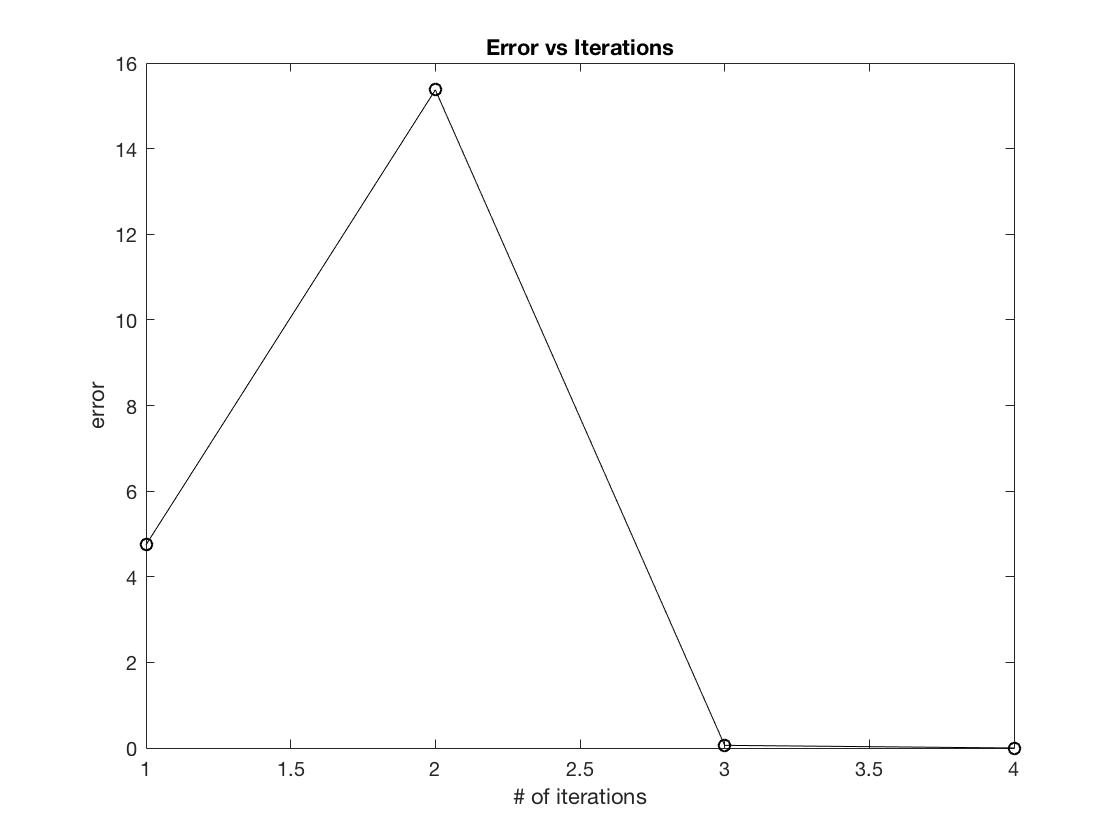
\includegraphics[scale = 0.35]{q4.jpg}\\\medskip
\end{center}
Compared to Secant method, Steffensen’s method requires the calculation of $f(x_{k}+f(x_{k}))$ while Secant method only evaluates $f(x_{k})$ within each iteration. Therefore, Secant is more efficient in terms of the required number of function evaluations.
 

\section{Question 5}
For this question, we also set the tolerance to be $10^{-4}$, the maximum iteration to be $10^{4}$. And $\alpha_{1} = -1$, $\alpha_{2} = 2$.
\paragraph{•$\phi(x) = x^{2}-1$}\mbox{}\\
Result: $\phi(x)$ doesn't converge.\\
\centerline{$\phi'(x) = 2x$}\\\linebreak
\centerline{$\phi'(\alpha_{1}) = -2$, $\phi'(\alpha_{2}) =4$}\\\linebreak
\centerline{$\mid(\phi'(\alpha_{1})\mid = 2>1$, $\mid(\phi'(\alpha_{2})\mid = 4>1$}\\\linebreak
Therefore, there is no convergence to $\alpha_{1}$ nor $\alpha_{2}$ with $\phi(x)$

\paragraph{•$\phi(x) = \sqrt{2+x}$}\mbox{}\\
Result: $\phi(x)$ only converges to $\alpha_{2}$.\\
\centerline{$\phi'(x) = \frac{1}{2}(2+x)^{-0.5}$}\\\linebreak
\centerline{$\phi'(\alpha_{1}) = \frac{1}{2} $, $\phi'(\alpha_{2}) = \frac{1}{4}$}\\\linebreak
\centerline{$\mid(\phi'(\alpha_{1})\mid =0.5< 1$, $\mid(\phi'(\alpha_{2})\mid = 0.25<1$}\\\linebreak
\centerline{However, $\phi(\alpha_{1}) \neq \alpha_{1}$}\\\linebreak
Therefore, it only converges to $\alpha_{2}$ with $\phi(x)$.

\paragraph*{•$\phi(x) = -\sqrt{2+x}$}\mbox{}\\
Result: $\phi(x)$ only converges to $\alpha_{1}$.\\
\centerline{$\phi'(x) = -\frac{1}{2}(2+x)^{-0.5}$}\\\linebreak
\centerline{$\phi'(\alpha_{1}) = -\frac{1}{2} $, $\phi'(\alpha_{2}) = -\frac{1}{4}$}\\\linebreak
\centerline{$\mid(\phi'(\alpha_{1})\mid =0.5< 1$, $\mid(\phi'(\alpha_{2})\mid = 0.25<1$}\\\linebreak
\centerline{However, $\phi(\alpha_{2}) \neq \alpha_{2}$}\\\linebreak
Therefore, it only converges to $\alpha_{1}$ with $\phi(x)$.

\paragraph*{•$\phi(x) = 1+\frac{2}{x}$}\mbox{}\\
Result: $\phi(x)$ only converges to $\alpha_{2}$.\\
\centerline{$\phi'(x) = \frac{-1}{x^{2}}$}\\\linebreak
\centerline{$\phi'(\alpha_{1}) = -1 $, $\phi'(\alpha_{2}) = \frac{-1}{4}$}\\\linebreak
\centerline{$\mid(\phi'(\alpha_{1})\mid =1$, $\mid(\phi'(\alpha_{2})\mid = \frac{-1}{4}<1$}\\\linebreak
Therefore, it only converges to $\alpha_{2}$ with $\phi(x)$.


\section{Question 6}
Mueller Method READ.

\end{document}
